\section{Основы uplift-моделирования}


\subsection{Склонность и чувствительность}

\iffalse
про продукты, про коммуникации и реакции на них, типы клиентов по реакциям
про модели склонности как основу всего и след уровень -- аплифт

    История возникновения аплифт моделирования.
    Основные понятия и определения.
    Отличия от традиционного моделирования.


------
\fi
Традиционно, при принятии решений на основе данных в бизнесе задаются вопросом вида <<Насколько конкретному клиенту интересен конкретный продукт?>>. Под интересом можно понимать вероятность (склонность) того, что клиент купит данный продукт (совершит целевое действие) без всякого воздействия на него. Таким образом, если знать для каждого клиента его вероятность покупки продукта, можно оценить число продаж по данному продукту и, соответственно, посчитать выручку. То есть так называемые склонностные модели полезны бизнесу для оценки экономики продукта. Но также эти модели могут помочь и в повышении эффективности маркетинговых кампаний: ведь зная, кто наиболее вероятно купит продукт даже без воздействия, мы можем его даже не предлагать остальным клиентам (тогда такую рекламу можно назвать таргетированной). Склонностные модели как раз и предсказывают для каждого клиента эту вероятность. В машинном обучении есть множество методов, предоставляющих возможность моделировать вероятность: логистическая регрессия, решающее дерево, случайный лес, градиентный бустинг.

Теперь допустим, что данный конкретный продукт становится более популярным, и клиенты начинают покупать его достаточно часто относительно изначального темпа продаж. Тогда встаёт вопрос не о том, кому его продавать в принципе, а о том, кому ещё его можно продать, пусть и с некоторой скидкой или дополнительным бонусом. Такой подход позволяет не найти целевую аудиторию для продукта, а расширить уже существующую, допустив при этом наличие некоторых воздействий на клиентов в виде скидок или бонусов. То есть теперь вопрос от бизнеса ставится следующим образом: <<Насколько сильнее конкретный клиент станет заинтересован в данном продукте при условии, что мы дадим ему скидку на него?>> Здесь под изменением интереса можно понимать изменение вероятности покупки продукта. Также это изменение интереса в результате некоторого воздействия на клиента можно называть его чувствительностью к этому воздействию, об оценке которой пойдёт речь далее в этой главе. Зная чувствительность всех клиентов, можно посчитать среднее увеличение прибыли в некоторой группе клиентов, у кого это изменение положительно (интерес вырос) и больше всего по модулю (они отреагировали на скидку ярче и сильнее остальных). Зная, какие клиенты реагируют на скидку положительнее всего, можно предлагать скидку только им, то есть сфокусироваться на клиентах, наиболее интересных с точки зрения бизнеса. Это позволит сделать маркетинговую кампанию эффективнее и сэкономить значительную сумму затрачиваемых средств.

При этом стоит отметить существенное отличие между понятиями склонности и чувствительности. Если склонность отвечает за вероятность того, что клиент купит данный продукт, то чувствительность отвечает за изменение этой вероятности при наличии конкретного воздействия относительно случая, когда этого воздействия не было. Это означает, что для оценки чувствительности клиента нужно:
\begin{itemize}
    \item жёстко фиксировать одно конкретное воздействие
    \item знать факт покупки клиентом продукта для обоих случаев наличия и отсутствия скидки
\end{itemize}

Заметим, что со вторым пунктом есть фундаментальная проблема: невозможно знать сразу оба исхода для одного клиента. Из этого следует, что напрямую измерить чувствительность для клиента мы не можем, и нужно оценивать её другими способами, о которых пойдёт речь далее в данной работе.

\iffalse
------
\fi













\iffalse

\subsection{АБ-тесты и uplift-моделирование}
связь с аб тестами ???
аплифт -- продвинутый персонализированный аб

    2.2. Основные принципы аплифт моделирования
    Принцип разности эффектов (Difference-in-Differences).
    Принцип двойного отбора (Double Selection).
    Принцип анализа случайных контрольных групп (Randomized Control Trials).

\fi














\subsection{Математическое определение uplift}

\iffalse
что такое аплифт математически
\fi

Введём некоторые обозначения, которые помогут нам записать формально общие соображения и требования к тому, что алгоритмы машинного обучения должны будут оптимизировать. Для начала нам понадобятся факты покупки клиентом продукта в случаях, когда скидка была и когда она отсутствовала, а также разность этих фактов:
\begin{itemize}
    \item $Y_i^0$ -- реакция клиента в случае, когда воздействия не было
    \item $Y_i^1$ -- реакция клиента в случае, когда воздействие было
    \item $\tau_i = Y_i^1 - Y_i^0$ -- разница реакций клиента в этих двух случаях, называемая causal effect
\end{itemize}

Заметим, что мы не можем знать одновременно $Y_i^0$ и $Y_i^1$, а потому и $\tau_i$ тоже, поэтому обучить модель прогнозировать напрямую $\tau_i$ мы не можем. Но если у нас есть признаковое описание клиента $X_i$, то можно ввести понятие CATE (Conditional Average Treatment Effect, условный усреднённый эффект от воздействия):
$$
    CATE = \mathbb{E} \left[ Y_i^1 | X_i \right] - \mathbb{E} \left[ Y_i^0 | X_i \right]
$$

Проблема CATE в том, что его невозможно пронаблюдать так же, как и $\tau_i$, поэтому не получится обучить модель предсказывать его. Однако, можно перейти к оценке CATE, которую и назовём uplift для конкретного клиента:
$$
    uplift_i = \widehat{CATE}_i = \mathbb{E} \left[ Y_i | X_i = x, W_i = 1 \right] - \mathbb{E} \left[ Y_i | X_i = x, W_i = 0 \right]
$$

Здесь были использованы два новых обозначения:
\begin{itemize}
    \item $W_i$ -- флаг воздействия на $i$-го клиента
    \item $Y_i = W_i Y_i^1 + (1 - W_i) Y_i^0$
\end{itemize}

Из обозначений выше следует, что $W_i = 1$ означает, что клиент попал в группу с воздействием (целевую), а $W_i = 0$ означает, что клиент попал в группу без воздействия (контрольную). Также при $W_i = 1$ выполнено $Y_i = Y_i^1$, а при $W_i = 0$ выполнено $Y_i = Y_i^0$.

Стоит отметить, что формулу для uplift для конкретного клиента можно записать только тогда, когда выполнено предположение о независимости назначений воздействий и признаковых описаний клиентов. То есть разбиение на контрольную и тестовую (целевую) группы не должно зависеть от значений какого-либо признака. Это условие называется CIA (Conditional Independence Assumption). Это важно, поскольку сами потенциальные реакции клиента $Y_i^0, Y_i^1$ в случаях наличия и отсутствия скидки определяются его признаковым описанием и не зависят от наличия данного воздействия. Но при этом сама наблюдаемая реакция $Y_i$, исходя из определения этой величины через $Y_i^0, Y_i^1$, уже зависит от наличия воздействия на объект.














\subsection{Правильное формирование выборки}

Из фундаментальной проблемы uplift-моделирования следует, что невозможно просто собрать выборку и обучить модель. Нас интересует разница между двумя взаимоисключающими случаями: случаем, когда клиент получил воздействие в виде скидки, и случаем, когда этого воздействия он не получил. Это значит, что на собираемые для построения моделей и проведения экспериментов данные нужно налагать некоторые особые требования. Как упоминалось выше, назначение воздействий не должно зависеть от какого-то конкретного признака или какого-то набора признаков. Это значит, что ещё до сбора различной информации о клиентах, нужно выбрать, кто именно получит скидку, а кто нет. Более того, это необходимо сделать случайным образом. После того, как выборки сформированы, нужно получить целевые переменные для обеих групп (и коктрольной, и целевой), при этом применив к целевой группе воздействие.

Здесь есть один важный момент, что между проводимым изначально экспериментом и последующей маркетинговой кампанией есть существенное различие: в эксперименте воздействие назначается случайным образом, а при проведении маркетинговой кампании нужно будет применять получившуюся uplift-модель и выбирать некоторый ТОП по её предсказаниям в качестве целевой группы. Если назначение воздействия в эксперименте происходит как-то иначе, то 

Также стоит помнить о том, что могли произойти какие-то внешние изменения, которые могли повлиять на распределения основных признаков в модели, поэтому при проведении самой маркетинговой компании на основе полученной модели, полезно также собрать и новые данные методом, аналогичным методу сбора данных для обучения модели. Это позволит, с одной стороны, оценить качество модели на новых данных относительно случайной модели, то есть понять, насколько проведённая маркетинговая кампания была эффективна на самом деле. Но с другой стороны это позволит не упустить момент для обновления модели на актуальных данных. На первый взгляд может показаться, что это не так важно, что можно было бы использовать для переобучения модели данные из самой кампании, но это не так. Если использовать данные из кампании, где для определения целевой группы использовалась модель, то назначение воздействий в этой группе будет не случайным, так как модель использует информацию о признаковом описании клиентов. То есть не будет выполнено свойство CIA, о котором говорилось ранее, и формулу для uplift использовать нельзя.















\subsection{Простейшие методы uplift-моделирования}

В этом разделе пойдёт речь о наиболее простых понятных методах моделирования uplift, которые в основном опираются на классическое определения uplift и на простые эвристики. Также в этом разделе содержится описание бейзлайна (базовой модели) для решения uplift-моделирования -- модели склонности.

Заметим, что предсказания модели используются для ранжирования объектов (в нашем случае клиентов банка) по величине чувствительности к воздействию. После сортировки по этой величине, для воздействия (или некоторой другой коммуникации) выберут некоторое количество клиентов сверху, то есть с наибольшими по величине значениями.

\subsubsection*{Бейзлайн}

Сначала обсудим базовое решение для задачи uplift-моделирования в виде модели склонности или же, другими словами, в виде обычного бинарного классификатора. Для ранжирования объектов необходимо, чтобы модель могла вернуть некоторое действительное число, это может быть оценка вероятности совершения клиентом целевого действия (в нашей конкретной задаче целевым действием является рефинансирование кредита наличными). После этого клиенты будут ранжироваться по этой вероятности и клиенты с максимальной вероятностью будут считаться максимально чувствительными к воздействию в виде скидки.

Данный способ моделирования может иметь некоторое интуитивное обоснование. Допустим, есть клиент с высоким уровнем склонности к рефинансированию кредита, тогда вполне вероятно, что он положительно отреагирует на скидку к процентной ставке. Ведь если человеку нужен кредит, то, увидев ставку пониже, он должен стать более уверенным в его взятии. Однако, как показывает практика, это далеко не всегда оправдано: если человек и так купил бы кредит, то давать ему скидку невыгодно с точки зрения бизнеса. То есть для бизнеса куда полезнее найти тех, кто изначально не так сильно склонен к рефинансированию, но со скидкой при этом стал более склонен. Из вышесказанного следует такая математическая запись для чувствительности:
$$
    uplift(x) = P(y | x)
$$

\subsubsection*{T-learner}

Перейдём к первому методу uplift-моделирования, который называется T-learner. Основная идея этого метода заключается в том, чтобы обучить две отдельные модели для каждой группы (целевой и контрольной). То есть одна модель будет обучена только на данных целевой группы, где воздействие было, и, таким образом, выучит зависимости в данных для этого случая. Другая же модель будет обучена только на данных контрольной группы, где не было никакого воздействия, и, таким образом, выучит зависимости в данных для этого случая. Тогда чувствительность можно выразить как разность этих двух вероятностей и использовать её для ранжирования клиентов. То есть для оценки чувствительности нового клиента нужно проскорить его моделью, обученной на данных выборки с воздействием, и моделью, обученной на данных выборки без воздействия, и затем вычесть второе из первого. Математически это можно записать так:
$$
    uplift(x) = P^T(x) - P^C(x)
$$
$$
    P^T(x) = P_1(y | x, W = 1), \: T = treatment
$$
$$
    P^C(x) = P_2(y | x, W = 0), \: C = control
$$

Здесть буквы $T$ и $C$ обозначают целевую и контрольную группы соответственно, а переменной $W$ обозначен флаг наличия воздействия на клиента. Разница между моделями показана с помощью индексов 1 и 2 у функций вероятности.

\subsubsection*{DDR/DFR}

Метод с двумя независимыми моделями (T-learner) кажется интуитивно понятным и правильным, но при этом сами модели не знают ничего о наличии воздействия на подаваемый им на вход объект, поэтому может возникнуть предположение, что добавление этой информации в одну из моделей некоторым образом может усилить их обе. Из этой идеи появился метод DDR (Dependent Data Representation) или DFR (Dependent Feature Representation) -- метод, который использует идею каскадов моделей, то есть основная идея в том, что сначала нужно обучить одну модель на одной группе (целевой или контрольной), затем сделать предсказания на второй группе и добавить предсказанные величины в качестве признака к текущему признаковому описанию объектов второй группы. При этом оценка чувствительности формируется так же, как в прошлых случаях. Это позволит учесть информацию из одной модели в другой и, возможно, улучшит качество итоговой модели. Формально для случая, когда предсказания модели, обученной на данных контрольной группы, подаются в модель, обученную на данных целевой группы, это можно записать следующим образом:
$$
    uplift(x) = P^T(x, P^C(x)) - P^C(x)
$$
$$
    P^T(x, P^C(x)) = P_1(y | x, P^C(x), W = 1), \: T = treatment
$$
$$
    P^C(x) = P_2(y | x, W = 0), \: C = control
$$

Однако, стоит заметить, что ровно так же можно подавать и предсказания модели, обученной на данных целевой группы, как дополнительный признак в модель, обученную на данных контрольной группы.

\subsubsection*{S-learner}

Теперь рассмотрим немного другой метод uplift-моделирования, который называется S-learner. Этот метод моделирования заключается в использовании обычной модели склонности, но при этом к признаковому описанию клиентов добавляется флаг наличия на этого клиента воздействия. Тогда предсказание, то есть оценка чувствительности, вычисляется снова как разность двух вероятностей, двух разных предсказаний для одного и того же клиента. Но теперь эти две вероятности получаются из одной и той же модели, обученной на модифицированной исходной выборке, с флагом воздействия, установленными сначала в 1, а затем в 0.

\iffalse 
Визуально модификацию выборки можно представить таким образом:

$$
\begin{matrix}
	\left(
	\begin{matrix}
    	  &  &   &  &  & \vline &   \\
    	  &  & X &  &  & \vline & y \\
    	  &  &   &  &  & \vline &   \\
	\end{matrix}
	\right)
\end{matrix}
\longrightarrow
\begin{matrix}
	\left(
	\begin{matrix}
    	  &  &   &  & \vline &   & \vline &   \\
    	  &  & X &  & \vline & W & \vline & y \\
    	  &  &   &  & \vline &   & \vline &   \\
	\end{matrix}
	\right)
\end{matrix}
$$

\fi

А записать предсказание математически можно следующим образом:
$$
    uplift(x) = P^T(x) - P^C(x)
$$
$$
    P^T(x) = P(y | x, W = 1), \: T = treatment
$$
$$
    P^C(x) = P(y | x, W = 0), \: C = control
$$

Здесь может показаться, что формула для T-learner точно такая же, но стоит заметить, что здесь нет никаких индексов у функций вероятности, поскольку используется лишь одна модель, просто с двумя разными флагами наличия воздействия $W$.

Есть один иногда полезный на практике трюк: добавить не только флаг воздействия в признаковое описание объекта, но и произведения этого флага со всеми изначально имеющимися признаками. В случае, если воздействие было и флаг равен 1, то это просто продублирует исходное признаковое описание в новые колонки. А если воздействия не было, то в новых колонках будут стоять нули.












\subsubsection*{Class Transformation}

Как должно быть понятно из названия, этот метод заключается в модификации целевой переменной. Основная идея метода в том, чтобы учесть в одной целевой переменной сразу оба флага -- и флаг наличия воздействия, и флаг совершения целевого действия, что позволит обучить стандартную модель, известную из классического машинного обучения. Предлагается ввести следующую переменную:
$$
    Z =
    \begin{cases}
        1, \text{ если } W = 1, \: Y = 1 \\
        1, \text{ если } W = 0, \: Y = 0 \\
        0, \text{ иначе }
    \end{cases},
$$

где $Z$ -- новая бинарная целевая переменная, $Y$ -- исходная бинарная целевая переменная, а $W$ -- флаг наличия воздействия, то есть $W, Y, Z \in \{0, 1\}$.

Эту формулу можно описать словами так: если реакция клиента при наличии воздействия не хуже, чем в случае отсутствия этого воздействия, то тогда присвоим этой переменной значение 1, а иначе присвоим значение 0. То есть значение 1 означает, что от наличия воздействия хуже не стало бы: если воздействия не было и целевое действие не было совершено, то от воздействия хуже стать не может, а вот лучше -- вполне (клиент может положительно отреагировать на наличие скидки), и также если было совершено целевое действие при наличии воздействия, то это означает, что в случае отсутствия воздействия результат мог бы стать только хуже (возможно, клиент не купил бы продукт, если бы мы не предоставили ему скидку).

Заметим, что формулу с рассмотрением случаев можно записать компактнее:
$$
    Z = Y \cdot W + (1 - Y) \cdot (1 - W)
$$

Но можно также заметить, что можно и ещё сократить запись:
$$
    Z = \mathbb{I}\{Y = W\}
$$

Для того, чтобы понять связь введённой нами величины $Z$ с uplift, полезно расписать выражение $P(Z=1 | X = x)$:
\begin{multline*}
    P(Z=1 | X = x) = \\
    = P(Z = 1 | X = x, W = 1) \cdot P(W = 1 | X = x) + \\
    P(Z = 1 | X = x, W = 0) \cdot P(W = 0 | X = x) = \\
    = P(Y = 1 | X = x, W = 1) \cdot P(W = 1 | X = x) + \\
    P(Y = 0 | X = x, W = 0) \cdot P(W = 0 | X = x)
\end{multline*}

Первое равенство было получено по формуле полной вероятности, где в качестве полной группы событий взяты противоположные события $W=0$ и $W=1$. А второе равенство получено исходя из формулы на $Z$ и условий в событиях с $Z, W$ в вероятностях. Теперь можно вспомнить предположение CIA, которое говорит о том, что вероятность для объекта попасть в целевую группу не должна зависеть от какого-либо его признака, то есть должно быть выполнено:
$$
    P(W | X = x) = P(W)
$$

Данное предположение позволяет упростить формулу для вероятности события $Z=1$, избавившись от зависимости от объекта:
\begin{multline*}
    P(Z=1 | X = x) = \\
    = P(Y = 1 | X = x, W = 1) \cdot P(W = 1) + \\
    P(Y = 0 | X = x, W = 0) \cdot P(W = 0)
\end{multline*}

Теперь можно заметить, что тут пригодятся введённые ранее обозначения для вероятностей целевого действия в контрольной и целевой группах:
\begin{gather*}
    P^T(Y = 1 | X = x) = P(Y = 1 | X = x, W = 1) \\
    P^C(Y = 1 | X = x) = P(Y = 1 | X = x, W = 0)
\end{gather*}

Учтя всё это, получим:
\begin{multline*}
    P(Z=1 | X = x) = \\
    = P^T(Y = 1 | X = x) \cdot P(W = 1) + \\
    P^C(Y = 0 | X = x) \cdot P(W = 0)
\end{multline*}

Теперь, рассмотрим один трюк, полезный на практике: предположим, что размеры контрольной и целевой групп равны. Это будет означать, что вероятность попасть в каждую из них будет равна $\frac{1}{2}$:
$$
    P(W = 1) = P(W = 0) = \frac{1}{2}
$$

Данное предположение позволяет написать следующее:
\begin{gather*}
    P(Z = 1 | X = x) =
        P^T(Y = 1 | X = x) \cdot \frac{1}{2} +
        P^C(Y = 0 | X = x) \cdot \frac{1}{2}
    \\
    2 \cdot P(Z = 1 | X = x) =
        P^T(Y = 1 | X = x) + 1 - P^C(Y = 1 | X = x)
    \\
    2 \cdot P(Z = 1 | X = x) - 1 =
        P^T(Y = 1 | X = x) - P^C(Y = 1 | X = x)
    \\
    2 \cdot P(Z = 1 | X = x) - 1 = uplift(x)
\end{gather*}

То есть, таким образом, для случая равных размеров целевой и контрольной групп можно использовать и такой способ моделирования uplift.























\subsection{Продвинутые методы uplift-моделирования}

X, R - learner, upllift tree, uplift rf, критерии информативности (LR, KL, ...)

Заметим, что методы, описанные в прошлой главе, довольно просты для понимания, но при этом они не учитывают некоторые тонкости, возникающие на практике, и которые могут влиять на точность обученных моделей. Поэтому стоит уделить внимание и другим, более сложным, методам uplift-моделирования, которые этим проблемы решают.

\subsubsection*{X-learner}

Этот метод аналогично методу DDR использует идею зависимости моделей через данные. Но если в DDR только предсказания одной из двух моделей подавались в другую, то здесь это верно для обеих моделей, поэтому зависимость между этими двумя моделями для X-learner иногда называется перекрёстной, что отражено в названии метода буквой X.

Данный метод решает проблему метода DDR, состоящую в том, что если целевая и контрольная группы имеют значительно отличающиеся размеры, то одна из моделей может быть недообучена, то есть её обощающая способность может быть низкой. В этом может помочь другая модель, обученная на другой группе и которая могла куда лучше уловить базовые зависимости между переменными. Идея состоит в том, чтобы использовать предсказания моделей друг в друге.

Если говорить о самом алгоритме, то он состоит из трёх основных этапов.























\subsection{Методы оценки качества uplift-моделей}

В этом разделе внимание будет уделено основным способам оценить качество uplift-модели. Мы рассмотрим как различные графики и диаграммы, так и привычные числовые метрики.

Поскольку задача uplift-моделирования преимущественно связана с сортировкой объектов по их чувствительности, то можно наблюдать некоторую аналогию с задачей ранжирования. Например, есть пороговые метрики, которые смотрят только на некоторый ТОП выборки по чувствительности, а есть общевыборочные метрики, которые учитывают все наблюдения. Мы рассмотрим оба типа метрик.



\subsubsection*{Метрика $uplift@k$}

Идея этой метрики состоим в следующем: нужно посмотреть по самым чувствительным клиентам, насколько увеличится конверсия от воздействия, то есть насколько чаще клиенты будут совершать целевое действие при наличии воздействия.

Данная метрика позволяет варьируя порог $k$ понять, какой эффект даст воздействие при применении его к разному числу клиентов, отранжированных по убыванию их чувствительности. Таким образом, бизнес сможет посчитать прибыль в каждом из наиболее интересных случаев и оценить, какому проценту от выборки выгоднее всего дать воздействие (например, скидку). Это важный вопрос, поскольку в каждом отдельном случае воздействие может иметь свою цену, иногда она может влечь довольно большие убытки.

Алгоритм подсчёта этой метрики довольно прост:
\begin{itemize}
    \item сортируем все объекты по убыванию прогнозной чувствительности
    \item берём ТОП $k\%$ выборки
    \item считаем среднюю конверсию в целевой группе 
    \item считаем среднюю конверсию в контрольной группе
    \item вычитаем вторую конверсию из первой
\end{itemize}

Математически это можно записать так:
$$
    uplift@k =
        \frac{
            \sum\limits_{i=1}^{kN} W_i Y_i
        }{
            \sum\limits_{i=1}^{kN} W_i
        }
        -
        \frac{
            \sum\limits_{i=1}^{kN} (1 - W_i) Y_i
        }{
            \sum\limits_{i=1}^{kN} (1 - W_i)
        }
    ,
$$

где использованы следующие обозначения:
\begin{itemize}
    \item $N$ -- размер выборки
    \item $k \in [ 0, 1 ]$ -- доля выборки для расчёта метрики
    \item $i$ -- номер объекта в порядке убывания чувствительности
    \item $W_i$ -- флаг наличия воздействия на $i$-го объекта
    \item $Y_i$ -- флаг того, своовершил ли $i$-й объект целевое действие
\end{itemize}

Стоит заметить, что теоретически область значений этой метрики совпадает с отрезком $[-1, 1]$. Метрика $uplift@k$ принимает значение -1 в том случае, когда в целевой группе никто не совершил целевого действия, а в контрольной группе все совершили целевое действие. Значение 1 эта метрика принимает в противоположном случае, когда в целевой группе все совершили целевое действие, а в контрольной группе никто не совершил целевого действия. На практике значение этой метрики обычно лежит от 0 до 1, но в зависимости от особенностей решаемой задачи, природы рассматриваемого конкретного воздействия и используемых данных метрика может принять и отрицательное значение для некоторых порогов $k$.




\subsubsection*{Диаграмма uplift by percentile}

Эта диаграмма является развитием идеи метрики $uplift@k$, и её можно представлять разными способами: как в виде таблицы, так и в виде графика. Эта диаграмма показывает, как сильно увеличилась конверсия в разных сегментах клиентов, полученных на основе их чувствительности к воздействию. Данный способ изображения информации об эффекте воздействия помогает лучше понять при разработке модели, куда смещён её фокус, а также он помогает при анализе результатов эксперимента понять, действительно ли не возникло ситуации, когда много чувствительных объектов было выделено в ТОП, но также значимая их доля оказалась вне выделенной части выборки.

\begin{figure}[ht]
\centering
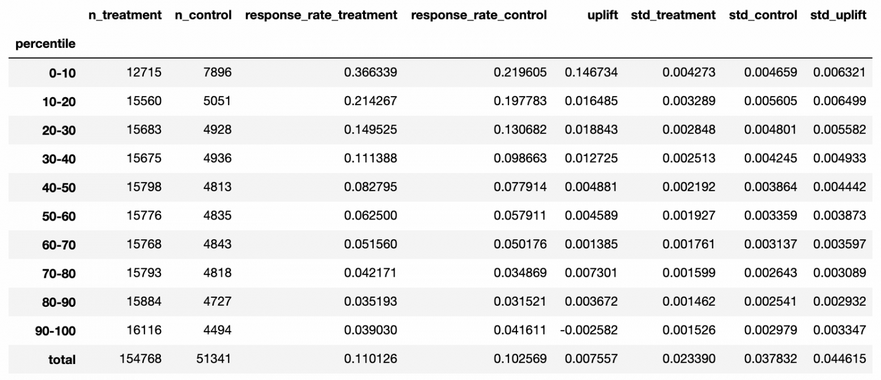
\includegraphics[scale=0.5]{pic_1_uplift_by_bins_table}
\centering
\caption{Таблица uplift by percentile для случая 10 бакетов}
\label{fig:pic_1_uplift_by_bins_table}
\end{figure}

Но так не очень понятен масштаб эффекта от воздействия в каждом сегменте, поэтому часто используют графический способ представить эту таблицу: он позволяет наглядно увидеть, насколько выше доля объектов, для которых целевое действие выполнено, при наличии воздействия, при этом сделать это сразу для каждого сегмента. На рисунке зелёные столбики означают среднюю долю объектов, совершивших целевое действие, в целевой группе, а жёлтые столбики означают среднюю долю объектов, совершивших целевое действие, в контрольной группе. Каждому столбику соответствует свой сегмент из того набора сегментов, которые получаются разбиением отсортированной выборки по предсказанному uplift.

\begin{figure}[ht]
\centering
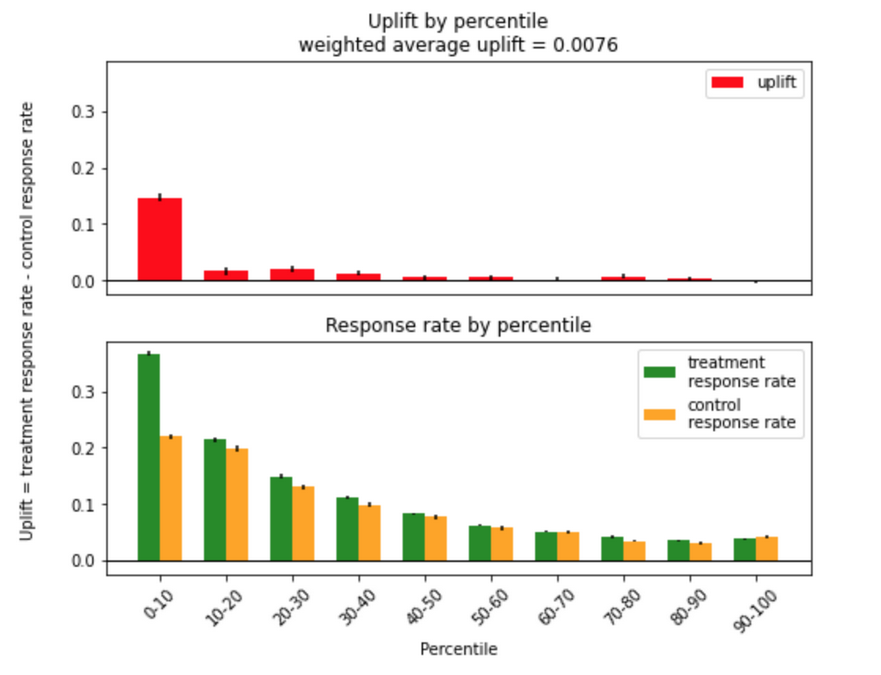
\includegraphics[scale=0.4]{pic_2_uplift_by_bins_graph}
\centering
\caption{График uplift by percentile для случая 10 бакетов}
\label{fig:pic_2_uplift_by_bins_graph}
\end{figure}

Для построения этой диаграммы нужно:
\begin{itemize}
    \item отсортировать все объекты по убыванию прогнозной чувствительности
    \item выбрать число сегментов (бинов, бакетов), на которое разбить выборку
    \item посчитать среднюю конверсию в каждом сегменте для целевой группы
    \item посчитать среднюю конверсию в каждом сегменте для контрольной группы
    \item посчитать их разницу в каждом сегменте
\end{itemize}

Чаще всего смотрят разбиение либо на 5, либо на 10 бакетов. Это связано с тем, что для достоверности и стабильности результатов нужно иметь в каждом бакете достаточное число наблюдений для того, чтобы иметь возможность обобщить результаты и выводы.

Стоит заметить, что также может быть полезно посмотреть для каждого сегмента на число наблюдений в контрольной и целевой частях этого сегмента. Это поможет проверить равномерное распределение обеих групп по бакетам. Распределение целевой и контрольных групп по бакетам должно быть примерно равномерным, поскольку оно зависит только от предсказанного uplift для каждого объекта. Если же количества наблюдений из контрольной и целевой групп в каждом бакете сильно отличаются, то это значит, что между предсказанной чувствительностью и наличием воздействия есть некоторая связь, чего быть не должно. Проблема заключается в том, что мы ожидаем выполнения предположения CIA, которое говорит о том, что наличие воздействия на объект не должно быть связано с каким-либо признаком этого объекта. И если мы предсказываем чувствительность клиента на основе данных контрольной и целевой групп, для признаков которых это предположение выполнено, то и у прогнозной чувствительности не должно быть информации о назначении воздействия. Более того, при предсказании uplift для новых объектов с целью найти наиболее чувствительных у нас этой информации нет. Это значит, что отсутствие равномерности распределения числа наблюдений из контрольной и целевой групп является достаточно веским основанием полагать, что эксперимент был проведён так, что воздействия назначались не произвольным образом и CIA не выполнено. Как обсуждалось ранее, это значит, что формула для uplift применена быть не может.

Также важно понимать, какой вид этой диаграммы хочется иметь. Цель uplift-моделирования в том, чтобы найти чувствительных клиентов, то есть тех, кто без воздействия имеет маленькую вероятность совершить целевое действие, а с воздействием -- большую. То есть в идеальном случае на диаграмме uplift by percentile зелёные столбики должны убывать по высоте, а жёлтые столбики должны возрастать по высоте.



\subsubsection*{Метрика weighted average uplift}

Эта метрика позволяет, с одной стороны, так же, как и $uplift@k$ иметь одно значение для описания качества моделей, по которому можно их сравнивать, но также эта метрика учитывает не только ТОП выборки по предсказаниям, а всю выборку целиком.

Здесь используется информация, полученная при построении табллицы uplift by percentile: идея метрики weighted average uplift состоит в том, чтобы взвесить uplift в каждом из бакетов на размеры частей этих бакетов, в которых находятся объекты из целевой группы, то есть те, к кому было применено воздействие. Математическая запись формулы выглядит так:
$$
    WAU = \frac{
        \sum\limits_{j=1}^{bins} N_j^T uplift_j
    }{
        \sum\limits_{j=1}^{bins} N_j^T
    }
    ,
$$
где:
\begin{itemize}
    \item $N_j^T$ -- число объектов с воздействием в $j$-ом бакете
    \item $uplift_j$ -- uplift в $j$-ом бакете
\end{itemize}

Теоретическое значение этой метрики лежит в отрезке от -1 до 1. Она равна 1 только тогда, когда во всех бакетах uplift равен 1, то есть целевое действие было совершено только в целевой группе, а в контрольной группе его не совершил никто. Получается, что высокие значения метрики означают, что без коммуникации или воздействия никто не будет совершать целевое действие (например, покупать продукт), и поэтому моделировать uplift может быть бесполезно. В таком случае полезнее моделировать вероятность совершения объектом целевого действия при воздействии, то есть сделать обычную модель склонности, но с учётом факта воздействия как некоторой данности. Такие модели называются response-моделями, поскольку они сразу предполагают наличие воздействия на объект и тем самым моделируют отклик на него (response). Значение -1, наоборот, означает, что при воздействии никто не будет совершать целевое действие, но такой случай нам не интересен: основная цель uplift-моделирования увеличить конверсию по высокочувствительным клиентам, а не уменьшить её. Поэтому наиболее интересный с точки зрения практики диапазон значений метрики лежит от 0 до 1.

Заметим, что если предположение CIA выполнено и целевая группа примерно равномерно распределена по бакетам, то weighted average uplift примерно равен среднему арифметическому uplift по всем бакетам.


\subsubsection*{Uplift-кривая}

Эта кривая показывает общее качество ранжирования uplift-моделью объектов по чувствительности. Для этого она считает накопительным итогом, проходя по всем возможным отсечкам ТОП объектов от 1 до размера выборки, средний uplift в выделенном ТОПе и умножает его на размер этого выделенного ТОПа. Получается, что в случае, когда воздействие представляет собой скидку, а наша цель состоит в приросте количества продаж, uplift-кривая показывает абсолютное число дополнительных продаж для данного ТОПа, если бы все клиенты в выделенном сегментв получили воздействие в виде скидки.

Математически формулу для uplift-кривой можно записать в краткой форме, с учётом определения $uplift@k$ ($N$ ниже -- размер выборки):

$$
    uplift-curve(t) = t \cdot uplift@ \left( \frac{t}{N} \cdot 100 \right)
$$

Также формулу можно расписать, подставив выражение для $uplift@k$ и разбив множитель $t$ на две суммы флагов принадлежности к контрольной и целевой группе (здесь используется то же обозначение $W_i$ для флага наличия воздействия, что и ранее в этой главе):
$$
    uplift-curve(t) =
        \left(
            \sum\limits_{i=1}^{t} W_i
            +
            \sum\limits_{i=1}^{t} (1 - W_i)
        \right)
        \cdot
        \left(
            \frac{
                \sum\limits_{i=1}^{t} W_i Y_i
            }{
                \sum\limits_{i=1}^{t} W_i
            }
            -
            \frac{
                \sum\limits_{i=1}^{t} (1 - W_i) Y_i
            }{
                \sum\limits_{i=1}^{t} (1 - W_i)
            }
        \right)
$$

Из этой формулы видно, что uplift-кривая всегда, независимо от порядка ранжирования объектов, заканчивается в точке, соответствующей общему приросту средней целевой переменной от воздействия на всю выборку. Это логично, поскольку если мы рассматриваем всю имеющуюся выборку, то скидки в таком случае были бы розданы всем клиентам, тогда от порядка их сортировки общий прирост продаж никак не поменяется. Заметим, что если рассмотреть пустую выборку, то есть ни к кому не применить воздействие (скидку), то прироста средней целевой переменной по выборке не будет, поэтому допустимо доопределить uplift-кривую нулём в точке $t=0$.

Обычно рисуют три uplift-кривые по аналогии с ROC-кривыми:
\begin{itemize}
    \item uplift-кривую для случайной модели
    \item uplift-кривую для обученной модели
    \item uplift-кривую для идеальной модели
\end{itemize}

Таким образом, из этих кривых можно понять, насколько лучше случайной модели наша модель выделяет чувствительные к воздействию объекты, а также насколько сильно она хуже идеальной модели. Причём чем выше uplift-кривая нашей модели над uplift-кривой случайной моделью, тем наша модель лучше.

Случайной моделью в данном случае является та модель, которая даёт прирост продаж, пропорциональный числу воздействий. Такого поведения мы и ждём, когда, например, произвольным образом раздаём клиентам скидки на определённый товар. Ведь логично ожидать, что чем больше клиентов получит скидку, тем больше клиентов купит товар. Из этого следует, что случайной моделью является та, у которой uplift-кривая идёт строго по прямой из точки $(0,0)$ в точку $(N, uplift-curve(N))$.

Идеальной моделью считается та, которая выше всех ставит всех чувствительных в положительном для воздействия и задачи смысле клиентов, затем нечувствительных, а затем чувствительных в негативном смысле. Но чтобы конкретно определить идеальный порядок, нужно знать для каждого клиента обе реакции (для случая, когда воздействие было и когда его не было), что невозможно, поэтому порядок для идеальной кривой определить достоверно невозможно, но можно определить порядок, который кажется логичным и разумным:
\begin{itemize}
    \item те, кто получил воздействие и совершил целевое действие
    \item те, кто НЕ получил воздействие и НЕ совершил целевое действие
    \item те, кто НЕ получил воздействие и совершил целевое действие
    \item те, кто получил воздействие и НЕ совершил целевое действие
\end{itemize}

\begin{figure}[ht]
\centering
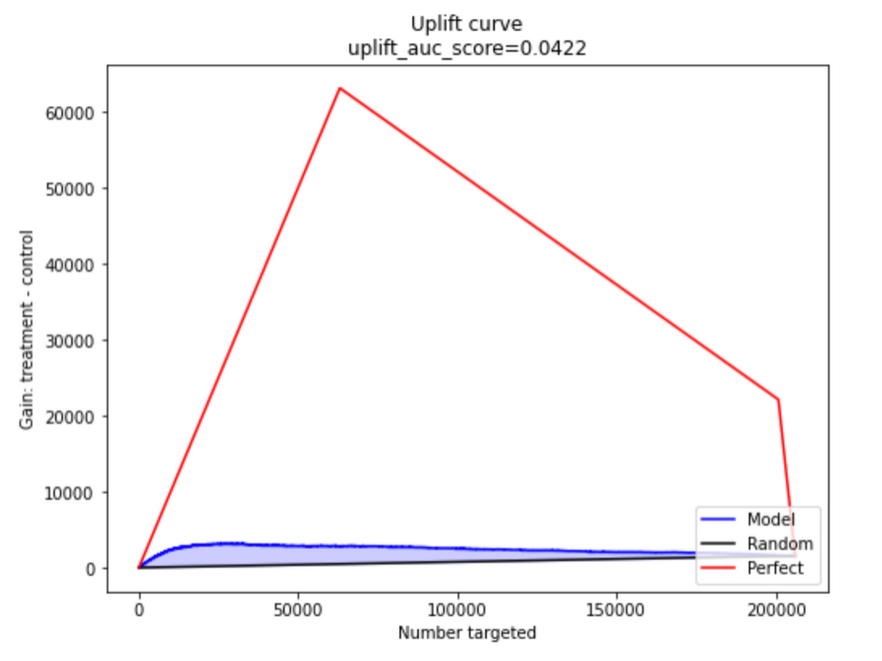
\includegraphics[scale=0.4]{pic_3_uplift_curve}
\centering
\caption{Uplift-кривые для случайной, типичной и идеальной моделей}
\label{fig:pic_3_uplift_curve}
\end{figure}


\subsubsection*{Qini-кривая}

Это ещё один распространённый тип графиков для оценки качества uplift-моделей, её формула довольно похоже на формулу для uplift-кривой, отличие состоит лишь в нормировке:
$$
    qini-curve(t) =
        \sum\limits_{i=1}^{t} W_i Y_i
        - 
        \frac{
            \sum\limits_{i=1}^{t} W_i
        }{
            \sum\limits_{i=1}^{t} (1 - W_i)
        }
        \sum\limits_{i=1}^{t} (1 - W_i) Y_i
$$

Эта кривая находится так же, как и uplift-кривая, накопительным итогом, причём для всех наблюдений. Также можно нарисовать qini-кривую для случайной модели и для идеальной модели. Аналогично с uplift-кривой, чем qini-кривая нашей модели выше над qini-кривой случайной моделью, тем наша модель лучше.

У qini-кривой есть некоторая интуиция, лежащая в её основе: если размер целевой группы сильно больше размера контрольной группы, то множитель в виде дроби из формулы выше будет увеличивать число совершённых целевых действий в контрольной группе до того же масштаба, что и число совершённых целевых действий в целевой группе, тем самым позволяя увидеть средний эффект от воздейстия в случае, когда размеры целевой и контрольной групп совпадают. Такая оценка более правдоподобна, чем просто разница в количествах совершённых целевых действий в обеих группах.

Можно заметить, что uplift-кривая выражается через qini-кривую простой нормировкой:
$$
    uplift-curve(t) = qini-curve(t) \frac{
        \sum\limits_{i=1}^{t} W_i
        +
        \sum\limits_{i=1}^{t} (1 - W_i)
    }{
        \sum\limits_{i=1}^{t} W_i
    }
$$

Из этой формулы видно, что в тех точках, где размеры контрольной и целевой групп одинаковы, значение uplift-кривой равно удвоенному значению qini-кривой. 

\begin{figure}[ht]
\centering
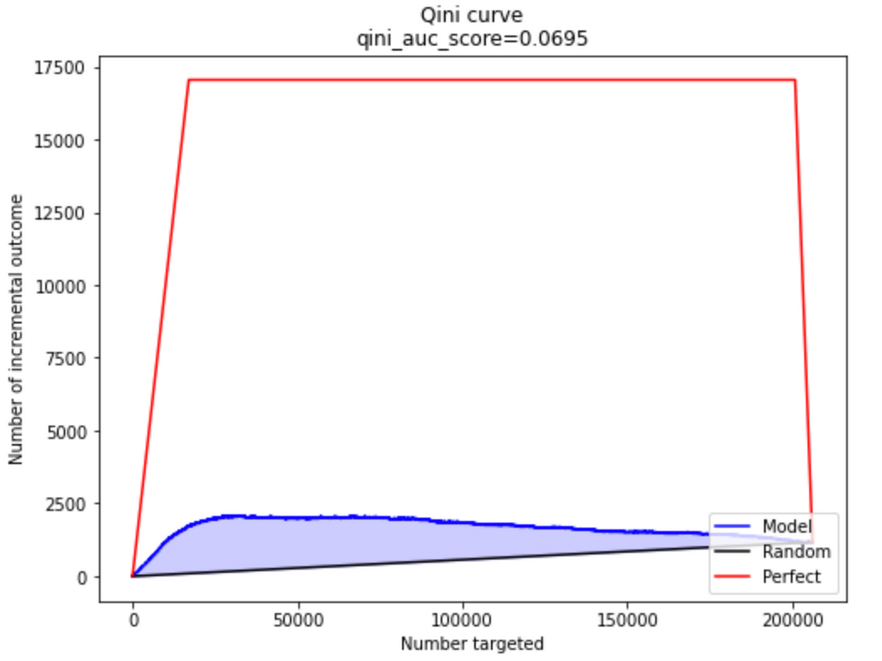
\includegraphics[scale=0.4]{pic_4_qini_curve}
\centering
\caption{Uplift-кривые для случайной, типичной и идеальной моделей}
\label{fig:pic_4_qini_curve}
\end{figure}


\subsubsection*{Метрики AUQC и AUUC}

Здесь так же, как и во многих задачах машинного обучения, полезно перейти от графиков к числам, и для графиков часто рассматривают плошадь под ними как единую меру качества модели. Площадь под кривой, отвечающей обученной нами модели, можно нормировать на площадь под кривой, овечающей идеальной модели, при этом вычтя из них обеих площадь под кривой, отвечающей случайной модели.

Таким образом, мы построим метрику AUQC (Area Under Qini Curve) или, как её ещё называют, Qini coefficient. Аналогично ей можно построить метрику AUUC (Area Under Uplift Curve), как отношение площадей под uplift-кривой нашей модели и uplift-кривой идеальной модели, из которых вычли площадь под uplift-кривой случайной модели.

\subsubsection*{Оценка калиброванности модели}

Часто немаловажным оказывается посмотреть не только на ранжирующую способность uplift-модели, но и на калиброванность её предсказаний. В случае uplift-моделирования предсказание модели обычно понимается как прирост конверсии продаж в ответ на некоторое воздействие на клиентов. Это значит, что uplift внутри выделенного сегмента, равный 0.05, означает, что в среднем при воздействии на этот сегмент продажи вырастут на 5\%. Если же реальный uplift, вычисленный как разница средних конверсий в целевой и контрольной группах, сильно отличается от 5\% и равен, например, 2\%, то положительный эффект от воздействия присутствует, но не в том объёме, в котором он ожидался. Поэтому крайне важно оценивать и калиброванность предсказаний uplift-моделей, поскольку это может повлиять на финансовые расчёты ожидаемой дополнительной прибыли от текущей маркетинговой кампании.

По аналогии с некоторыми прошлыми метриками и диаграммами, логично рассмотреть разбиение на бакеты внутри выборки и вычислить разницу между средними целевыми переменными в контрольной и целевой частях каждого бакета этой выборки. Перед этим нужно, естественно, выборку отсортировать по предсказанным величинам, описывающим чувствительность объектов. Аналогичным образом необходимо разбить на бакеты сами предсказанные чувствительности. Тогда будет возможно сравнить точность предсказанных эффектов от воздействия на сегмент с реальным наблюдаемым эффектом от этого воздействия. Эти отличия во всех бакетах можно дальше описать одним числом, например, с помощью стандартных метрик регрессии: средняя квадратичная ошибка, средняя абсолютная ошибка, коэффициент детерминации. Сложностью данного метода является выбор числа бакетов, на которые нужно разбить выборку, поскольку при малом их числе будет трудно заметить какой-либо эффект от воздействия, а при слишком большом числе бакетов есть риск того, что размеры самих бакетов будут слишком малы для статистически значимых выводов, поэтому нельзя будет утверждать, что эффектв данном бакете вообще есть. 




















\subsection{Примеры применения uplift-моделирования}

    Маркетинг и рекламные кампании.
    Медицинские исследования.
    Финансовые услуги и страхование.
    Социальные и поведенческие науки.

Чуть подробнее стоит обсудить области, где может быть применено uplift-моделирование. Поскольку uplift -- это оценка эффекта от некоторого воздействия на объект, то обсужденные выше методы можно применять везде, где есть такое воздействие, причём вне зависимости от его природы. Основными областями, где применяются подобные методы являются:
\begin{itemize}
    \item бизнес
    \item финансы
    \item медицина
\end{itemize}

Если говорить о бизнесе, то основными примерами здесь являются продуктовые и маркетинговые кампании. Здесь важно уметь определять чувствительных к воздействию клиентов для экономии ресурсов компании. Нецелесообразное их использование может повлечь заметные убытки и даже уменьшить размер клиентской базы из-за коммуникации с теми клиентами, с которыми она была нежелательна. Также важно уметь находить среди клиентов, которые хотят перестать пользоваться услугами компании, тех, кто согласен остаться, хоть и с определёнными льготами или более выгодными условиями.

В финансовом секторе похожая ситуация: например, в банках крайне важно решать задачи привлечения клиентов, их развития в среде банка и их удержании, когда есть основания полагать, что клиент собирается перестать пользоваться усугами банка. Для этого могут быть полезны различные воздействия: для растранзачивания клиента можно предложить ему дополнительный кэшбэк, а для удержания, например, дополнительный пакет услуг или дополнительные преимущества.

Теперь перейдем к медицине, в которой часто возникают ситуации, когда для нового разработанного лекарства нужно оценить степень влияния на человеческий организм. В данной ситуации важно понять, кто подвержен развитию побочных заболеваний, кто действительно выздоровеет от использования данного препарата, а кто не восприимчив к нему и продолжит болеть. Также можно выделить для разных вариантов лекарства наиболее подходящих ему пациентов, чтобы дать им наиболее подходящий.















\subsection{Проблемы uplift-моделирования}

Несмотря на развитие методов uplift-моделирования в течение долгого времени (более 30 лет) и поднятие в научных публикациях различных вопросов из этой области, до сих пор эта область кажется недостаточно исследованной. Например, не было найдено исследований на темы:
\begin{itemize}
    \item насколько модели склонности хуже uplift-моделей?
    \item насколько полезны методы отбора признаков в uplift-моделировании?
    \item что делать с проблемой переобучения uplift-моделей?
    \item что делать с проблемой калиброванности uplift-моделей?
    \item можно ли применить градиентный бустинг для uplift-моделирования?
\end{itemize}

Каждый из этих вопросов довольно сложен, и на первые два попытается ответить данная работа. Но это далеко не все проблемы, связанные с предсказанием uplift. Например, как эффективно работать со случаем множества воздействий и выбирать на основе прогнозов чувствительности лучшее их них? Или как исключить накопительный эффект в цепочке воздействий с некоторым интервалом, то есть какого временного промежутка достаточно, чтобы считать, что эффект от прошлого воздействия стал незначительным?

По мере развития направления uplift-моделирования будут проявляться новые тонкости, проблемы, задачи, а также предлагаться новые методы их решения.










\iffalse

\begin{figure}[ht]
\minipage{0.475\textwidth}
  \centering
$$
\left(
\begin{array}{cc|c}
\color{red!30}{1} & \cdots & 2 \\ 
\vdots & \ddots & 2 \\
\color{red!70}{1} & 6 & 2 \\ 
\end{array}
\right)
$$
\caption{Квадрки}
\label{fig:quadr}
\endminipage
\minipage{0.475\textwidth}
  \centering
$$
\left(
\begin{array}{cc|c}
\color{red!30}{1} & \cdots & 2 \\ 
\vdots & \ddots & 2 \\
\color{red!70}{1} & 6 & 2 \\ 
\end{array}
\right)
$$
\caption{Квадрки}
\label{fig:quadr}
\endminipage
\end{figure}













\begin{figure}[ht]
\minipage{0.775\textwidth}
  \centering
$$
\left(
\begin{array}{cc|c}
\color{red!30}{1} & \cdots & 2 \\ 
\vdots & \ddots & 2 \\
\color{red!70}{1} & 6 & 2 \\ 
\end{array}
\right)
$$
\caption{Квадрки}
\label{fig:quadr}
\endminipage
\end{figure}












\begin{itemize}
\setlength{\itemindent}{0.25in}
    \item
    \item
    \item
\end{itemize}







\begin{figure}[h]
\includegraphics[scale=0.5]{hash_buckets}
\centering
\end{figure}






\begin{figure}[ht]
\minipage{0.475\textwidth}
  \centering
$$
\left(
\begin{array}{cc|c}
\color{red!30}{1} & \cdots & 2 \\ 
\vdots & \ddots & 2 \\
\color{red!70}{1} & 6 & 2 \\ 
\end{array}
\right)
$$
\caption{Квадрки}
\label{fig:quadr}
\endminipage
\end{figure}





\fi

